\documentclass[8pt]{article}
\usepackage[margin=1in]{geometry}
\usepackage[all]{xy}


\usepackage{amsmath,amsthm,amssymb,color,latexsym}
\usepackage{geometry}        
\geometry{letterpaper}    
\usepackage{graphicx}

\usepackage{listings}
\usepackage{xcolor}

\usepackage[export]{adjustbox}

\definecolor{codegreen}{rgb}{0,0.6,0}
\definecolor{codegray}{rgb}{0.5,0.5,0.5}
\definecolor{codepurple}{rgb}{0.58,0,0.82}
\definecolor{backcolour}{rgb}{0.95,0.95,0.92}

\lstdefinestyle{mystyle}{
  backgroundcolor=\color{backcolour},   commentstyle=\color{codegreen},
  keywordstyle=\color{magenta},
  numberstyle=\tiny\color{codegray},
  stringstyle=\color{codepurple},
  basicstyle=\ttfamily\footnotesize,
  breakatwhitespace=false,         
  breaklines=true,                 
  captionpos=b,                    
  keepspaces=true,                 
  numbers=left,                    
  numbersep=5pt,                  
  showspaces=false,                
  showstringspaces=false,
  showtabs=false,                  
  tabsize=2
}

\lstset{style=mystyle}

\usepackage{graphicx}
\graphicspath{ {./images/} }


\newtheorem{problem}{Problem}

\newenvironment{solution}[1][\it{Solution}]{\textbf{#1. } }{$\square$}


\begin{document}
\noindent CS 6140: Machine Learning Spring 2021\hfill Homework Assignment \#2\\
Sai Nikhil (02/27/2021)\hfill thirandas.s@northeastern.edu

\hrulefill


\begin{problem}
Naive Bayes classifier. Consider a binary classification problem where there are eight data points in the training set. That is,
$$
\begin{aligned}
\mathcal{D}=\{(-1,-1,-1,-),(-1,-1,1,+),(-1,1,-1,+),(-1,1,1,-),\\(1,-1,-1,+),(1,-1,1,-),(1,1,-1,-),(1,1,1,+)\}
\end{aligned}
$$
where each tuple $\left(x_{1}, x_{2}, x_{3}, y\right)$ represents a training example with input vector $\left(x_{1}, x_{2}, x_{3}\right)$ and class label $y$\\
a) (10 points) Construct a naive Bayes classifier for this problem and evaluate its accuracy on the training set. Measure accuracy as the fraction of correctly classified examples.\\
b) (10 points) Transform the input space into a higher-dimensional space
$$
\left(x_{1}, x_{2}, x_{3}, x_{1} x_{2}, x_{1} x_{3}, x_{2} x_{3}, x_{1} x_{2} x_{3}, x_{1}^{2}, x_{2}^{2}, x_{3}^{2}, x_{1}^{2} x_{2}, x_{1} x_{2}^{2}, x_{1} x_{3}^{2}, x_{2}^{2} x_{3}, x_{2} x_{3}^{2}\right)
$$
and repeat the previous step.\\
Carry out all steps manually and show all your calculations. Discuss your main observations.
\end{problem}
\begin{solution}
\\

\textbf{a)}\\

Let us re-order and write the training set as follows,
$$
\begin{array}{|c|c|c|c|}
\hline x_{1} & x_{2} & x_{3} & y \\
\hline-1 & -1 & -1 & - \\
\hline-1 & 1 & 1 & - \\
\hline 1 & -1 & 1 & - \\
\hline 1 & 1 & -1 & - \\
\hline-1 & -1 & 1 & + \\
\hline-1 & 1 & -1 & + \\
\hline 1 & -1 & -1 & + \\
\hline 1 & 1 & 1 & + \\
\hline
\end{array}
$$

The input vector and class label are both discrete in this case. We have, $\mathcal{X}_{j} = \{-1, 1\} \text { and } \mathcal{Y} = \{-, +\}$.

The posterior for a class is given by,

$$
\begin{aligned}
p(y \mid \boldsymbol{x}) \propto p(\boldsymbol{x} \mid y) p(y)
\end{aligned}
$$

After applying Naive Bayes assumption, we have,
$$
p\left(x_{1}, x_{2}, \ldots, x_{d} \mid y\right)=\prod_{j=1}^{d} p\left(x_{j} \mid y\right)
$$

We know that class conditional is given by,

$$
    P(X_{j} = l | Y = k) = \frac{\text{\# times } X_{j} = l \wedge Y = k}{\text{\# times } Y = k} = \frac{m_{j,l,k}}{n_k}
$$

In order to avoid $\frac{0}{0}$ issues, we can evaluate class conditional using smoothing, where the smoothing parameter $\ell = 1$. The new form of class conditional thus becomes,

$$
    P(X_{j} = l | Y = k) = \frac{m_{j,l,k} + \ell}{n_k + \ell|\mathcal{X}_j|} = \frac{m_{j,l,k} + 1}{n_k + 2}
$$

From the training data, the class conditionals are as follows:

$$
\begin{aligned}
    P(X_{1} = -1 | Y = -) = \frac{2 + 1}{4 + 2} = \frac{1}{2}\\
    P(X_{1} = 1 | Y = -) = \frac{2 + 1}{4 + 2} = \frac{1}{2}\\
    P(X_{1} = -1 | Y = +) = \frac{2 + 1}{4 + 2} = \frac{1}{2}\\
    P(X_{1} = 1 | Y = +) = \frac{2 + 1}{4 + 2} = \frac{1}{2}\\
    P(X_{2} = -1 | Y = -) = \frac{2 + 1}{4 + 2} = \frac{1}{2}\\
    P(X_{2} = 1 | Y = -) = \frac{2 + 1}{4 + 2} = \frac{1}{2}\\
    P(X_{2} = -1 | Y = +) = \frac{2 + 1}{4 + 2} = \frac{1}{2}\\
    P(X_{2} = 1 | Y = +) = \frac{2 + 1}{4 + 2} = \frac{1}{2}\\
    P(X_{3} = -1 | Y = -) = \frac{2 + 1}{4 + 2} = \frac{1}{2}\\
    P(X_{3} = 1 | Y = -) = \frac{2 + 1}{4 + 2} = \frac{1}{2}\\
    P(X_{3} = -1 | Y = +) = \frac{2 + 1}{4 + 2} = \frac{1}{2}\\
    P(X_{3} = 1 | Y = +) = \frac{2 + 1}{4 + 2} = \frac{1}{2}\\
\end{aligned}
$$

The class probability after applying smoothing is of the form,

$$
    P(Y = k) = \alpha_k = \frac{n_k + \ell}{n + \ell|\mathcal{Y}|} = \frac{n_k + 1}{n + 2}
$$

The class probabilities are,

$$
    P(Y = -) = \frac{4 + 1}{8 + 2} = \frac{1}{2} \,\,\,\,\,\,\,\text{and}\,\,\,\,\,\,\, P(Y = +) = \frac{4 + 1}{8 + 2} = \frac{1}{2}
$$

Therefore,

$$
\begin{aligned}
    P(\boldsymbol{x} = (-1, -1, -1) | Y = -) &= \prod_{j=1}^{3} P(X_j = -1 | Y = -)\\
    &= P(X_1 = -1 | Y = -) \times P(X_2 = -1 | Y = -) \times P(X_3 = -1 | Y = -)\\
    &= \frac{1}{2} \times \frac{1}{2} \times \frac{1}{2} = \frac{1}{8}
\end{aligned}
$$

Similarly,
$$
\begin{aligned}
    P(\boldsymbol{x} = (-1, 1, 1) | Y = -) = \frac{1}{8}\\
    P(\boldsymbol{x} = (1, -1, 1) | Y = -) = \frac{1}{8}\\
    P(\boldsymbol{x} = (1, 1, -1) | Y = -) = \frac{1}{8}\\
    P(\boldsymbol{x} = (-1, -1, 1) | Y = +) = \frac{1}{8}\\
    P(\boldsymbol{x} = (-1, 1, -1) | Y = +) = \frac{1}{8}\\
    P(\boldsymbol{x} = (1, -1, -1) | Y = +) = \frac{1}{8}\\
    P(\boldsymbol{x} = (1, 1, 1) | Y = +) = \frac{1}{8}\\
\end{aligned}
$$

Let, $P(\boldsymbol{x}) = k$. Hence the posteriors are,

$$
\begin{aligned}
    P(Y = - | \boldsymbol{x} = (-1, -1, -1)) &= \frac{P(\boldsymbol{x} = (-1, -1, -1) | Y = -) \times P(Y = -)}{P(\boldsymbol{x})}\\
    &= \frac{\frac{1}{8} \times \frac{1}{2}}{k}\\
    &= \frac{1}{16k}
\end{aligned}
$$

Similarly,
$$
\begin{aligned}
    P(Y = - | \boldsymbol{x} = (-1, 1, 1)) &= \frac{1}{16k}\\
    P(Y = - | \boldsymbol{x} = (1, -1, 1)) &= \frac{1}{16k}\\
    P(Y = - | \boldsymbol{x} = (1, 1, -1)) &= \frac{1}{16k}\\
    P(Y = + | \boldsymbol{x} = (-1, -1, 1)) &= \frac{1}{16k}\\
    P(Y = + | \boldsymbol{x} = (-1, 1, -1)) &= \frac{1}{16k}\\
    P(Y = + | \boldsymbol{x} = (1, -1, -1)) &= \frac{1}{16k}\\
    P(Y = + | \boldsymbol{x} = (1, 1, 1)) &= \frac{1}{16k}\\
\end{aligned}
$$

and the complementary posterior probabilities are,

$$
\begin{aligned}
    P(Y = + | \boldsymbol{x} = (-1, -1, -1)) &= \frac{1}{16k}\\
    P(Y = + | \boldsymbol{x} = (-1, 1, 1)) &= \frac{1}{16k}\\
    P(Y = + | \boldsymbol{x} = (1, -1, 1)) &= \frac{1}{16k}\\
    P(Y = + | \boldsymbol{x} = (1, 1, -1)) &= \frac{1}{16k}\\
    P(Y = - | \boldsymbol{x} = (-1, -1, 1)) &= \frac{1}{16k}\\
    P(Y = - | \boldsymbol{x} = (-1, 1, -1)) &= \frac{1}{16k}\\
    P(Y = - | \boldsymbol{x} = (1, -1, -1)) &= \frac{1}{16k}\\
    P(Y = - | \boldsymbol{x} = (1, 1, 1)) &= \frac{1}{16k}\\
\end{aligned}
$$

We classify a dataset $\boldsymbol{x}$ as $+$ if, $P(Y = + | \boldsymbol{x}) > P(Y = - | \boldsymbol{x})$, else we classify it with $-$.

With that logic, the first 4 training examples in the re-ordered set in the above table are classified correctly with a $-$. Rest all are incorrectly classified.

Hence, the accuracy = $\frac{4}{8} \times 100 \% = 50 \%$.
\\

\textbf{b)}

The training data is,


$$
\begin{array}{|c|c|c|c|c|c|c|c|c|c|c|c|c|c|c|c|}
\hline x_{1} & x_{2} & x_{3} & x_{4} & x_{5} & x_{6} & x_{7} & x_{8} & x_{9} & x_{10} & x_{11} & x_{12} & x_{13} & x_{14} & x_{15} & y \\
\hline-1 & -1 & -1 & 1 & 1 & 1 & -1 & 1 & 1 & 1 & -1 & -1 & -1 & -1 & -1 & - \\
\hline-1 & 1 & 1 & -1 & -1 & 1 & -1 & 1 & 1 & 1 & 1 & -1 & -1 & 1 & 1 & - \\
\hline 1 & -1 & 1 & -1 & 1 & -1 & -1 & 1 & 1 & 1 & -1 & 1 & 1 & 1 & -1 & - \\
\hline 1 & 1 & -1 & 1 & -1 & -1 & -1 & 1 & 1 & 1 & 1 & 1 & 1 & -1 & 1 & - \\
\hline-1 & -1 & 1 & 1 & -1 & -1 & 1 & 1 & 1 & 1 & -1 & -1 & -1 & 1 & -1 & + \\
\hline-1 & 1 & -1 & -1 & 1 & -1 & 1 & 1 & 1 & 1 & 1 & -1 & -1 & -1 & 1 & + \\
\hline 1 & -1 & -1 & -1 & -1 & 1 & 1 & 1 & 1 & 1 & -1 & 1 & 1 & -1 & -1 & + \\
\hline 1 & 1 & 1 & 1 & 1 & 1 & 1 & 1 & 1 & 1 & 1 & 1 & 1 & 1 & 1 & + \\
\hline
\end{array}
$$

In the above table,

$$
\begin{aligned}
x_4 = x_{1} x_{2}, x_5 = x_{1} x_{3}, x_6 = x_{2} x_{3}, x_7 = x_{1} x_{2} x_{3}, x_8 = x_{1}^{2}, x_9 = x_{2}^{2},\\
x_{10} = x_{3}^{2}, x_{11} = x_{1}^{2} x_{2}, x_{12} = x_{1} x_{2}^{2}, x_{13} = x_{1} x_{3}^{2}, x_{14} = x_{2}^{2} x_{3}, x_{15} = x_{2} x_{3}^{2}
\end{aligned}
$$

Let, $$P(X_{j} = l | Y = k) = \alpha_{j,l,k}$$

Therefore,

$$
\begin{array}{|c|c|c|c|c|c|c|c|c|c|c|c|c|c|c|c|}
\hline & \alpha_{1} & \alpha_{2} & \alpha_{3} & \alpha_{4} & \alpha_{5} & \alpha_{6} & \alpha_{7} & \alpha_{8} & \alpha_{9} & \alpha_{10} & \alpha_{12} & \alpha_{12} & \alpha_{13} & \alpha_{14} & \alpha_{15} \\
\hline X_j = -1, Y = - & \frac{1}{2} & \frac{1}{2} & \frac{1}{2} & \frac{1}{2} & \frac{1}{2} & \frac{1}{2} & \frac{5}{6} & \frac{1}{6} & \frac{1}{6} & \frac{1}{6} & \frac{1}{2} & \frac{1}{2} & \frac{1}{2} & \frac{1}{2} & \frac{1}{2} \\
\hline X_j = -1, Y = + & \frac{1}{2} & \frac{1}{2} & \frac{1}{2} & \frac{1}{2} & \frac{1}{2} & \frac{1}{2} & \frac{1}{6} & \frac{1}{6} & \frac{1}{6} & \frac{1}{6} & \frac{1}{2} & \frac{1}{2} & \frac{1}{2} & \frac{1}{2} & \frac{1}{2} \\
\hline X_j = 1, Y = - & \frac{1}{2} & \frac{1}{2} & \frac{1}{2} & \frac{1}{2} & \frac{1}{2} & \frac{1}{2} & \frac{1}{6} & \frac{5}{6} & \frac{5}{6} & \frac{5}{6} & \frac{1}{2} & \frac{1}{2} & \frac{1}{2} & \frac{1}{2} & \frac{1}{2} \\
\hline X_j = 1, Y = + & \frac{1}{2} & \frac{1}{2} & \frac{1}{2} & \frac{1}{2} & \frac{1}{2} & \frac{1}{2} & \frac{5}{6} & \frac{5}{6} & \frac{5}{6} & \frac{5}{6} & \frac{1}{2} & \frac{1}{2} & \frac{1}{2} & \frac{1}{2} & \frac{1}{2} \\
\hline
\end{array}
$$


The class probabilities are,

$$
    P(Y = -) = \frac{4 + 1}{8 + 2} = \frac{1}{2} \,\,\,\,\,\,\,\text{and}\,\,\,\,\,\,\, P(Y = +) = \frac{4 + 1}{8 + 2} = \frac{1}{2}
$$

Let $P(\boldsymbol{x}) = k$ $\forall \boldsymbol{x}$.

Therefore,

$$
\begin{aligned}
P(Y = - | \boldsymbol{x} = (-1, -1, -1, 1, 1, 1, -1, 1, 1, 1, -1, -1, -1, -1, -1)) &= \frac{P(\boldsymbol{x} | Y = -) \times P(Y = -)}{P(\boldsymbol{x})}\\
&= \frac{\frac{1}{2^{11}}\times\frac{5^4}{6^4}\times\frac{1}{2}}{k}\\
&= \frac{5^4}{2^{12} \times 6^4k}
\end{aligned}
$$

and

$$
\begin{aligned}
P(Y = + | \boldsymbol{x} = (-1, -1, -1, 1, 1, 1, -1, 1, 1, 1, -1, -1, -1, -1, -1)) &= \frac{\frac{1}{2^{11}}\times\frac{5^3}{6^4}\times\frac{1}{2}}{k}\\
&= \frac{5^3}{2^{12} \times 6^4k}
\end{aligned}
$$

Therefore from above two equations for first vector, $P(Y = + | \boldsymbol{x}) \le P(Y = - | \boldsymbol{x})$.

$\implies$ The vector should be classified as $-$, which is as given.

For second vector,

$$
\begin{aligned}
P(Y = - | \boldsymbol{x}) &= \frac{\frac{1}{2^{11}}\times\frac{5^4}{6^4}\times\frac{1}{2}}{k}\\
&= \frac{5^4}{2^{12} \times 6^4k}
\end{aligned}
$$

$$
\begin{aligned}
P(Y = + | \boldsymbol{x}) &= \frac{\frac{1}{2^{11}}\times\frac{5^3}{6^4}\times\frac{1}{2}}{k}\\
&= \frac{5^3}{2^{12} \times 6^4k}
\end{aligned}
$$

Here also, $P(Y = + | \boldsymbol{x}) \le P(Y = - | \boldsymbol{x}) \implies$ The vector should be classified as $-$, which is as given.


For third and fourth vectors,

$$
\begin{aligned}
P(Y = - | \boldsymbol{x}) &= \frac{\frac{1}{2^{11}}\times\frac{5^4}{6^4}\times\frac{1}{2}}{k}\\
&= \frac{5^4}{2^{12} \times 6^4k}
\end{aligned}
$$

$$
\begin{aligned}
P(Y = + | \boldsymbol{x}) &= \frac{\frac{1}{2^{11}}\times\frac{5^3}{6^4}\times\frac{1}{2}}{k}\\
&= \frac{5^3}{2^{12} \times 6^4k}
\end{aligned}
$$

Here also, $P(Y = + | \boldsymbol{x}) \le P(Y = - | \boldsymbol{x}) \implies$ The vector should be classified as $-$, which is as given.\\


For fifth, sixth, seventh and eighth vectors,

$$
\begin{aligned}
P(Y = + | \boldsymbol{x}) &= \frac{\frac{1}{2^{11}}\times\frac{5^4}{6^4}\times\frac{1}{2}}{k}\\
&= \frac{5^4}{2^{12} \times 6^4k}
\end{aligned}
$$

$$
\begin{aligned}
P(Y = - | \boldsymbol{x}) &= \frac{\frac{1}{2^{11}}\times\frac{5^3}{6^4}\times\frac{1}{2}}{k}\\
&= \frac{5^3}{2^{12} \times 6^4k}
\end{aligned}
$$

Here, $P(Y = + | \boldsymbol{x}) > P(Y = - | \boldsymbol{x}) \implies$ The vector should be classified as $+$, which is as given.

Hence, the accuracy = $\frac{8}{8} \times 100 \% = 100 \%$.\\\\

\textbf{Observations:}\\

\begin{enumerate}
\item Clearly the feature $x_7 = x_1x_2x_3$ is alone enough to classify input vectors correctly with $100 \%$ accuracy in case b).
\item Features $x_2^2$ and $x_3^2$ are redundant as they as produce the same output as $x_1^2$. Similarly, $x_1^2x_2$ is same as $x_2$, $x_1x_2^2$ and $x_1x_3^2$ are same as $x_1$, $x_2^2x_3$ is same as $x_3$, $x_2x_3^2$ is same as $x_2$. Such redundant features should be removed while performing Naive Bayes classification. However, in this special case, their presence doesn't effect the classification.
\end{enumerate}

\end{solution}



\begin{problem}
Consider a binary classification problem in which we want to determine the optimal decision surface. A point $\mathrm{x}$ is on the decision surface if $P(Y=1 \mid \mathrm{x})=P(Y=0 \mid \mathrm{x})$.\\

a) (10 points) Find the optimal decision surface assuming that each class-conditional distribution is defined as a two-dimensional Gaussian distribution:
$$
p(\mathbf{x} \mid Y=i)=\frac{1}{(2 \pi)^{d / 2}\left|\boldsymbol{\Sigma}_{i}\right|^{1 / 2}} \cdot e^{-\frac{1}{2}\left(\mathbf{x}-\mathbf{m}_{i}\right)^{T} \boldsymbol{\Sigma}_{i}^{-1}\left(\mathbf{x}-\mathbf{m}_{i}\right)}
$$
where $i \in\{0,1\}, \mathbf{m}_{0}=(1,2), \mathbf{m}_{1}=(6,3), \mathbf{\Sigma}_{0}=\mathbf{\Sigma}_{1}=\mathbf{I}_{2}, P(Y=0)=P(Y=1)=\frac{1}{2}, \mathbf{I}_{d}$ is the d-dimensional identity matrix, and $\left|\boldsymbol{\Sigma}_{i}\right|$ is the determinant of $\boldsymbol{\Sigma}_{i}$.\\

b) (5 points) Generalize the solution from part (a) using $\mathbf{m}_{0}=\left(m_{01}, m_{02}\right), \mathbf{m}_{1}=\left(m_{11}, m_{12}\right), \mathbf{\Sigma}_{0}=\mathbf{\Sigma}_{1}= \sigma^{2} \mathbf{I}_{2}$ and $P(Y=0) \neq P(Y=1)$.

c) (10 points) Generalize the solution from part (b) to arbitrary covariance matrices $\boldsymbol{\Sigma}_{0}$ and $\boldsymbol{\Sigma}_{1} .$ Discuss the shape of the optimal decision surface.
\end{problem}

\begin{solution}
\\

\textbf{a)}\\

For optimal decision surface, we have, $P(Y=0 \mid \mathbf{x})=P(Y=1 \mid \mathbf{x})$.

$$
\text { Let, } \mathbf{x} =\left[\begin{array}{l}
x_{1} \\
x_{2}
\end{array}\right]
$$

Therefore,

\begin{align*}
P(\mathbf{x} \mid Y = 0) \cdot P(Y = 0) &= P(\mathbf{x} \mid Y = 1) \cdot P(Y = 1)\\
\implies \frac{1}{(2 \pi)^{d / 2}\left|\boldsymbol{\Sigma}_{0}\right|^{1 / 2}} \cdot e^{-\frac{1}{2}\left(\mathbf{x}-\mathbf{m}_{0}\right)^{T} \boldsymbol{\Sigma}_{0}^{-1}\left(\mathbf{x}-\mathbf{m}_{0}\right)} \cdot \frac{1}{2} &= \frac{1}{(2 \pi)^{d / 2}\left|\boldsymbol{\Sigma}_{1}\right|^{1 / 2}} \cdot e^{-\frac{1}{2}\left(\mathbf{x}-\mathbf{m}_{1}\right)^{T} \boldsymbol{\Sigma}_{1}^{-1}\left(\mathbf{x}-\mathbf{m}_{1}\right)} \cdot \frac{1}{2}\\
\implies (x_1 - 1)^2 + (x_2 - 2)^2 &= (x_1 - 6)^2 + (x_2 - 3)^2\\
\end{align*}
$$
\boxed{5x_1+x_2 = 20}
$$


\textbf{b)}\\

Let, $P(Y=0) = \alpha \text{ and } P(Y=1) = 1 - \alpha$\\

Therefore,
\begin{align*}
P(\mathbf{x} \mid Y = 0) \cdot P(Y = 0) &= P(\mathbf{x} \mid Y = 1) \cdot P(Y = 1)\\
\frac{1}{(2 \pi)^{d / 2}\left|\boldsymbol{\Sigma}_{0}\right|^{1 / 2}} \cdot e^{-\frac{1}{2}\left(\mathbf{x}-\mathbf{m}_{0}\right)^{T} \boldsymbol{\Sigma}_{0}^{-1}\left(\mathbf{x}-\mathbf{m}_{0}\right)} \cdot \alpha &= \frac{1}{(2 \pi)^{d / 2}\left|\boldsymbol{\Sigma}_{1}\right|^{1 / 2}} \cdot e^{-\frac{1}{2}\left(\mathbf{x}-\mathbf{m}_{1}\right)^{T} \boldsymbol{\Sigma}_{1}^{-1}\left(\mathbf{x}-\mathbf{m}_{1}\right)} \cdot (1 - \alpha)\\
\implies (x_1-m_{01})^2 + (x_2-m_{02})^2 - (x_1-m_{11})^2 - (x_1-m_{12})^2 &= 2 \sigma^2 \ln\left(\frac{\alpha}{1 - \alpha}\right)\\
\end{align*}
$$
\boxed{(m_{11} - m_{01}) x_1 + (m_{12} - m_{02}) x_2 + \frac{(m_{01}^2 + m_{02}^2 - m_{11}^2 - m_{12}^2)}{2} - \sigma^2 \ln\left(\frac{\alpha}{1 - \alpha}\right) = 0}
$$


\textbf{c)}\\

Generalizing the above equation, we get,

\begin{align*}
e^{\frac{\left(\mathbf{x} - \mathbf{m}_{0}\right)^{T} \mathbf{\Sigma}_{0}^{-1}\left(\mathbf{x}-\mathbf{m}_{0}\right) - \left(\mathbf{x}-\mathbf{m}_{1}\right)^{T} \mathbf{\Sigma}_{1}^{-1}\left(\mathbf{x}-\mathbf{m}_{1}\right)}{2}}&=\frac{\alpha}{1 - \alpha} \sqrt{\frac{\left|\mathbf{\Sigma}_{1}\right|}{\left|\mathbf{\Sigma}_{0}\right|}}
\end{align*}
$$
\left(\mathbf{x} - \mathbf{m}_{0}\right)^{T} \mathbf{\Sigma}_{0}^{-1}\left(\mathbf{x}-\mathbf{m}_{0}\right) - \left(\mathbf{x}-\mathbf{m}_{1}\right)^{T} \mathbf{\Sigma}_{1}^{-1}\left(\mathbf{x}-\mathbf{m}_{1}\right) - 2 \ln\left(\frac{\alpha}{1 - \alpha} \sqrt{\frac{\left|\mathbf{\Sigma}_{1}\right|}{\left|\mathbf{\Sigma}_{0}\right|}}\right)= 0
$$

Upon substituting constants, this will be simplified to the form,
$$
\boxed{Ax_1^2+Bx_2^2+Cx_1x_2+Dx_1+Ex_2+F = 0}
$$

\begin{center}
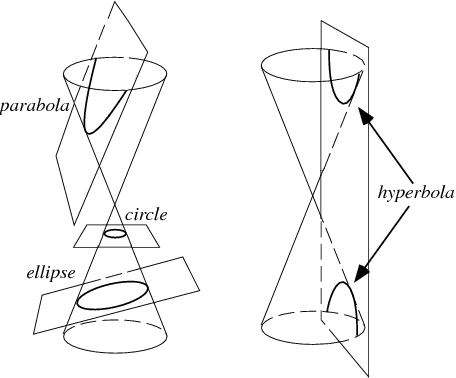
\includegraphics[width=10cm, keepaspectratio]{ConicSection}
\end{center}

This is the generic equation of a conic section in a 2-D plane as shown above. The shape of the conic will depend on following values:

$$
\begin{array}{l}
\Delta=\left|\begin{array}{ccc}
A & \frac{1}{2} C & \frac{1}{2} D \\
\frac{1}{2} C & B & \frac{1}{2} E \\
\frac{1}{2} D & \frac{1}{2} E & F
\end{array}\right|, \quad J=\left|\begin{array}{cc}
A & \frac{1}{2} C \\
\frac{1}{2} C & B
\end{array}\right|, \quad I=A+B, \\\\
K=\left|\begin{array}{cc}
A & \frac{1}{2} D \\
\frac{1}{2} D & F
\end{array}\right|+\left|\begin{array}{cc}
B & \frac{1}{2} E \\
\frac{1}{2} E & F
\end{array}\right|
\end{array}
$$

The appropriate cases for different conics are given below:

$$
\begin{array}{ccccl}
\Delta & J & \Delta / 1 & K & \text { Type of conic } \\
\hline \neq 0 & <0 & & & \text { hyperbola } \\
\neq 0 & 0 & & & \text { parabola } \\
\neq 0 & >0 & <0 & & \text { ellipse } \\
\neq 0 & >0 & >0 & & \text { (imaginary ellipse) } \\
0 & <0 & & & \text { intersecting lines } \\
0 & >0 & & & \text { point } \\
0 & 0 & & <0 & \text { distinct parallel lines } \\
0 & 0 & & >0 & \text { (imaginary parallel lines) } \\
0 & 0 & & 0 & \text { coincident lines }
\end{array}
$$


\end{solution}





\begin{problem}
Problem 3. (55 points) Consider a multivariate linear regression problem of mapping $\mathbb{R}^{d}$ to $\mathbb{R}$, with two different objective functions. The first objective function is the sum of squared errors, as presented in class;
i.e., $\sum_{i=1}^{n} e_{i}^{2},$ where $e_{i}=w_{0}+\sum_{j=1}^{d} w_{j} x_{i j}-y_{i} .$ The second objective function is the sum of square Euclidean distances to the hyperplane; i.e., $\sum_{i=1}^{n} r_{i}^{2},$ where $r_{i}$ is the Euclidean distance between point $\left(x_{i}, y_{i}\right)$ to the hyperplane $f(x)=w_{0}+\sum_{j=1}^{d} w_{j} x_{j}$.\\

a) (10 points) Derive a gradient descent algorithm to find the parameters of the model that minimizes the sum of squared errors.\\

b) (20 points) Derive a gradient descent algorithm to find the parameters of the model that minimizes the sum of squared distances.\\

c) (20 points) Implement both algorithms and test them on 3 datasets. Datasets can be randomly generated, as in class, or obtained from resources such as UCI Machine Learning Repository. Compare the solutions to the closed-form (maximum likelihood) solution derived in class and find the $R^{2}$ in all cases on the same dataset used to fit the parameters; i.e., do not implement cross-validation. Briefly describe the data you use and discuss your results.\\

d) (5 points) Normalize every feature and target using a linear transform such that the minimum value for each feature and the target is 0 and the maximum value is $1 .$ The new value for feature $j$ of data point $i$ can be found as
$$
x_{i j}^{\text {new }}=\frac{x_{i j}-\min _{k \in\{1,2, \ldots, n\}} x_{k j}}{\max _{k \in\{1,2, \ldots, n\}} x_{k j}-\min _{k \in\{1,2, \ldots, n\}} x_{k j}}
$$
where $n$ is the dataset size. The new value for the target $i$ can be found as
$$
y_{i}^{\text {new }}=\frac{y_{i}-\min _{k \in\{1,2, \ldots, n\}} y_{k}}{\max _{k \in\{1,2, \ldots, n\}} y_{k}-\min _{k \in\{1,2, \ldots, n\}} y_{k}}
$$
Measure the number of steps towards convergence and compare with the results from part (c). Briefly discuss your results.
\end{problem}

\begin{solution}\\

\textbf{a)}\\

\textbf{Given:} A set of observations
$$
D=\left\{\left(x_{i}, y_{i}\right)\right\}_{i=1}^{n},\left(x_{i,} y_{i}\right) \in \mathbb{R}^{d} \times \mathbb{R}
$$

\textbf{Objective:} Find best linear approximator
$$
f(x)=\omega_{0}+\sum_{j=1}^{d} \omega_{j} x_{j}
$$

Minimize sum of squares = $\sum_{i=1}^{n}\left(f\left(x_{i}\right)-y_{i}\right)^{2}$\\

\textbf{Rewrite:} Minimize,
$$
SSE=\sum_{i=1}^{n}\left(w_{0}+\sum_{j=1}^{d} w_{j} x_{i j}-y_{i}\right)^{2}
$$

Suppose, $\boxed{x_{i 0}=1}$,
$$
SSE\left(w_{0}, w_{1}, \cdots w_{d}\right)=\sum_{i=1}^{n}\left(\sum_{j=0}^{d} w_{j} x_{i j}-y_{i}\right)^{2}
$$

Writing in vector form, we get,
$$
\boxed{SSE(\mathbf{w}) = \left(\mathbf{xw}-\mathbf{y}\right)^T\left(\mathbf{xw}-\mathbf{y}\right)}
$$

Hence,
$$
\boxed{\nabla SSE(\mathbf{w})=2\mathbf{x}^{T}\left(\mathbf{xw}-\mathbf{y}\right)}
$$

For gradient descent,
$
\mathbf{w}^{(t+1)}=\mathbf{w}^{(t)}-\eta \cdot \nabla SSE\left(\mathbf{w}^{(t)}\right)
$, where $\eta \in(0,1]$ \\

$$
\boxed{\mathbf{w}^{(t+1)}=\mathbf{w}^{(t)}-2 \eta \mathbf{x}^{T}\left(\mathbf{xw}^{(t)}-\mathbf{y}\right)}
$$


\textbf{b)}\\

\textbf{Given:} A set of observations
$$
D=\left\{\left(x_{i}, y_{i}\right)\right\}_{i=1}^{n},\left(x_{i,} y_{i}\right) \in \mathbb{R}^{d} \times \mathbb{R}
$$

\textbf{Objective:} Find best linear approximator
$$
f(x)=\omega_{0}+\sum_{j=1}^{d} \omega_{j} x_{j}
$$


Minimize sum of squared euclidian distances,
$$
\begin{aligned}
SSED &=\sum_{i=1}^{n}\frac{(f\left(x_{i}\right)-y_{i})^2}{\|\mathbf{w}\|^2+1} \\
&= \sum_{i=1}^{n} \frac{\left(w_{0}+\sum_{j=1}^{d} w_{j} x_{i}-y_{i}\right)^{2}}{\|\mathbf{w}\|^{2}+1}
\end{aligned}
$$

Suppose, $\boxed{x_{i0}=1}$, \\
$$
\begin{aligned}
SSED(w_0, w_1, \cdots w_d) &=\sum_{i=1}^{n} \frac{\left(\sum_{j=0}^{d} w_{j} x_{i j}-y_{i}\right)^{2}}{\|w\|^{2}+1} \\
&=\frac{\sum_{i=1}^{n}\left(\sum_{j=0}^{d} w_{j} x_{i j}-y_{i}\right)^{2}}{\sum_{k=1}^{d} w_{k}^{2}+1} \\
&=\frac{S S E\left(w_{0}, w_{1}, \ldots w_{d}\right)}{\sum_{k=1}^{d} w_{k}^{2}}
\end{aligned}
$$

$$
\implies \boxed{SSED(\mathbf{w}) = \frac{SSE(\mathbf{w})}{\|\mathbf{w}\|^2+1}}
$$

Hence,
$$
\begin{aligned}
\frac{\partial(SSED)}{\partial w_{0}}&=\frac{\left(\sum_{k=1}^{d} w_{k}^{2}+1\right) \times \frac{\partial}{\partial w_{0}}(SSE) - SSE \times 0}{\left(\sum_{k=1}^{d} w_{k}^{2}+1\right)^{2}}
\end{aligned}
$$

and,  when $1 \le p \le d$,
$$
\frac{\partial(SSED)}{\partial w_{p}}=\frac{\left(\sum_{k=1}^{d} w_{k}^{2}+1\right) \times \frac{\partial(SSE)}{\partial w_{P}} - SSE \times \left(2 w_{p}\right)}{\left(\sum_{k=1}^{d} w_{k}^{2}+1\right)^{2}}
$$

We modify $\mathbf{w}$ vector by putting, $w_0 = 0$ to get $\mathbf{w}_2$,

Hence,
$$
\boxed{\nabla SSED (\mathbf{w}, \mathbf{w}_2) =\frac{\left(\|\mathbf{w}_2\|^{2} + 1\right) \times \nabla SSE(\mathbf{w}) - 2 \times SSE(\mathbf{w}) \times \mathbf{w}_2}{\left(\|\mathbf{w}_2\|^{2}+1\right)^2}}
$$

Let for $\mathbf{t}^{th}$ step, the modified $\mathbf{w}^{(t)}$ be ${\mathbf{w}_2}^{(t)}$.

So, for gradient descent,
$
\mathbf{w}^{(t+1)}=\mathbf{w}^{(t)}-\eta \cdot \nabla SSED\left({\mathbf{w}}^{(t)}, {\mathbf{w}_2}^{(t)}\right)
$, where $\eta \in(0, 1]$ \\

$$
\boxed{\mathbf{w}^{(t+1)}=\mathbf{w}^{(t)}-\eta \left(\frac{\left(\|{\mathbf{w}_2}^{(t)}\|^{2}+1\right) \times \nabla SSE({\mathbf{w}}^{(t)}) - 2 \times SSE({\mathbf{w}}^{(t)}) \times {\mathbf{w}_2}^{(t)}}{\left(\|{\mathbf{w}_2}^{(t)}\|^2+1\right)^{2}}\right)}
$$

\textbf{c) \& d)}\\

For code, please look into \textbf{GradientDescent.ipynb}.\\

\textbf{Output:}\\
\\
1)\\
Actual weights =  [1 2] \\
WARNING: Convergence not obtained for <function SSED at 0x7fd54d030b80>\\
Raw dataset results:\\
Weights from Maximum Likelihood = [1.25499004 1.98981147] \\
Weights from Sum of Squared Error = [1.25888602 1.98237399] Number of iterations taken =  336 \\
Weights from Sum of Squared Euclidean Distance Error = [1.79207960e-03 4.21289384e+00] Number of iterations taken =  100000 \\
$R^2$ for Maximum Likelihood = 0.9423719488680293 \\
$R^2$ for Sum of Squared Error = 0.9423585914916401 \\
$R^2$ for Sum of Squared Euclidean Distance Error = -0.3125292809590352 \\
\\
WARNING: Convergence not obtained for <function SSED at 0x7fd54d030b80>\\
Normalized dataset results:\\
Weights from Maximum Likelihood = [0.08428984 0.82866939] \\
Weights from Sum of Squared Error = [0.080403   0.83608681] Number of iterations taken =  232 \\
Weights from Sum of Squared Euclidean Distance Error = [0.00183914 0.9647496 ] Number of iterations taken =  100000 \\
$R^2$ for Maximum Likelihood = 0.9405070723861864 \\
$R^2$ for Sum of Squared Error = 0.9404306160582103 \\
$R^2$ for Sum of Squared Euclidean Distance Error = 0.9110184877290902 \\
\\
2)\\
Actual weights =  [1 2 3] \\
WARNING: Convergence not obtained for <function SSED at 0x7fd54d030b80>\\
Raw dataset results:\\
Weights from Maximum Likelihood = [1.23021267 2.02393632 3.01567512] \\
Weights from Sum of Squared Error = [1.23897042 2.01566028 3.00716707] Number of iterations taken =  411 \\
Weights from Sum of Squared Euclidean Distance Error = [9.11827650e-04 3.10726850e+00 4.17204299e+00] Number of iterations taken =  100000 \\
$R^2$ for Maximum Likelihood = 0.9810229751608907 \\
$R^2$ for Sum of Squared Error = 0.981012314928364 \\
$R^2$ for Sum of Squared Euclidean Distance Error = 0.7807863494298954 \\

WARNING: Convergence not obtained for <function SSED at 0x7fd54d030b80>\\
Normalized dataset results:\\
Weights from Maximum Likelihood = [0.02130786 0.40205078 0.5999009 ] \\
Weights from Sum of Squared Error = [0.01296103 0.41063084 0.60728349] Number of iterations taken =  326 \\
Weights from Sum of Squared Euclidean Distance Error = [3.44419144e-04 4.20719822e-01 6.19044100e-01] Number of iterations taken =  100000 \\
$R^2$ for Maximum Likelihood = 0.9815491309587564 \\
$R^2$ for Sum of Squared Error = 0.9813044292617724 \\
$R^2$ for Sum of Squared Euclidean Distance Error = 0.9800893873012639 \\
\\
3)\\
Actual weights =  [1 2 3 4] \\
WARNING: Convergence not obtained for <function SSED at 0x7fd54d030b80>\\
Raw dataset results:\\
Weights from Maximum Likelihood = [1.23175493 2.00920529 3.02320381 4.00696197] \\
Weights from Sum of Squared Error = [1.24252118 2.00268153 3.01665139 3.99957899] Number of iterations taken =  544 \\
Weights from Sum of Squared Euclidean Distance Error = [4.19130419e-04 2.71024299e+00 3.76068168e+00 4.83138405e+00] Number of iterations taken =  100000 \\
$R^2$ for Maximum Likelihood = 0.9915521623406103 \\
$R^2$ for Sum of Squared Error = 0.9915472787565527 \\
$R^2$ for Sum of Squared Euclidean Distance Error = 0.9292159669387261 \\

WARNING: Convergence not obtained for <function SSED at 0x7fd54d030b80>\\
Normalized dataset results:\\
Weights from Maximum Likelihood = [-0.09614229  0.25250589  0.37625801  0.50156219] \\
Weights from Sum of Squared Error = [-0.1068754   0.25926529  0.38285911  0.5086211 ] Number of iterations taken =  410 \\
Weights from Sum of Squared Euclidean Distance Error = [-0.00150743  0.19394194  0.32020437  0.44452522] Number of iterations taken =  100000 \\
$R^2$ for Maximum Likelihood = 0.9915165897073519 \\
$R^2$ for Sum of Squared Error = 0.9912062933639023 \\
$R^2$ for Sum of Squared Euclidean Distance Error = 0.9681003338416297 \\
\\
4)\\
+++++++++++++START WITH N = 300 and D = 15+++++++++++++\\
Actual weights =  [1 2 4 4 2 4 4 1 4 2 4 5 1 1 2 3] \\
WARNING: Convergence not obtained for <function SSE at 0x7fd54d030700>\\
WARNING: Convergence not obtained for <function SSED at 0x7fd54d030b80>\\
Raw dataset results:\\
Weights from Maximum Likelihood = [1.11379202 2.00029796 3.99977594 4.00013072 2.00049968 4.00002218
 3.99985206 1.0002666  4.00036985 1.9999127  3.99993452 5.00038289
 1.00011637 1.00009822 2.00048834 3.00036932] \\
Weights from Sum of Squared Error = [6.55525175e+303             inf             inf             inf
             inf             inf             inf             inf
             inf             inf             inf             inf
             inf             inf             inf             inf] Number of iterations taken =  91 \\
Weights from Sum of Squared Euclidean Distance Error = [-9.01336498e-06 -1.37630440e+02  4.59005871e+02 -8.54542452e+01
  1.48951236e+03  3.87126499e+02  7.20603366e+02  9.57736517e+02
 -4.30511843e+02  2.89074535e+02 -1.68475555e+03 -3.16648651e+02
 -4.24806071e+02 -6.64258165e+02 -1.77869449e+02  8.49412333e+01] Number of iterations taken =  100000 \\
$R^2$ for Maximum Likelihood = 0.9999998167501309 \\
$R^2$ for Sum of Squared Error = nan \\
$R^2$ for Sum of Squared Euclidean Distance Error = -60694.73590778983 \\
\\
WARNING: Convergence not obtained for <function SSED at 0x7fd54d030b80>\\
Normalized dataset results:\\
Weights from Maximum Likelihood = [-0.34941459  0.08970206  0.18447254  0.18363183  0.09199215  0.18160336
  0.18226469  0.04420227  0.18116071  0.09201079  0.18117562  0.22684705
  0.0449425   0.0456999   0.09390231  0.13825206] \\
Weights from Sum of Squared Error = [-0.44835348  0.09889455  0.19320891  0.19519339  0.11112236  0.19363335
  0.19811723  0.06018336  0.19083287  0.10666284  0.1936614   0.24515874
  0.05618911  0.05946077  0.10792598  0.14598463] Number of iterations taken =  2354 \\
Weights from Sum of Squared Euclidean Distance Error = [-0.00040218  0.05428484  0.1527442   0.14297237  0.02808748  0.14070359
  0.13078585 -0.01279373  0.14730324  0.04002846  0.13681534  0.16844793
  0.00216292 -0.0042922   0.04477235  0.1073495 ] Number of iterations taken =  100000 \\
$R^2$ for Maximum Likelihood = 0.9983488145823171 \\
$R^2$ for Sum of Squared Error = 0.9901491922153589 \\
$R^2$ for Sum of Squared Euclidean Distance Error = 0.8965566890039539 \\
\\
++++++++++++++++++++END+++++++++++++++++++++\\
\\
5)\\
+++++++++++++START WITH N = 300 and D = 25+++++++++++++\\
Actual weights =  [1 3 2 5 2 5 4 1 3 1 3 1 4 4 4 3 1 3 5 3 5 5 3 5 3 3] \\
WARNING: Convergence not obtained for <function SSE at 0x7fd54d030700>\\
WARNING: Convergence not obtained for <function SSED at 0x7fd54d030b80>\\
Raw dataset results:\\
Weights from Maximum Likelihood = [1.22925544 2.99969538 2.00006519 5.00030685 1.99979471 5.00023927
 4.00007528 1.00006182 3.00008527 0.99998621 2.99981107 0.99994666
 3.99955583 4.00009405 4.00028369 2.99966477 0.99996969 2.99997628
 4.9998824  3.00034224 5.00004925 5.00005719 3.00025455 5.00035179
 3.00024262 2.99992421] \\
Weights from Sum of Squared Error = [-inf -inf -inf -inf -inf -inf -inf -inf -inf -inf -inf -inf -inf -inf
 -inf -inf -inf -inf -inf -inf -inf -inf -inf -inf -inf -inf] Number of iterations taken =  86 \\
Weights from Sum of Squared Euclidean Distance Error = [ 2.51767061e-06 -9.88697125e+02  9.00873261e+01 -1.92963409e+03
 -2.35525810e+02 -6.63291427e+00  3.39117084e+02  1.23302792e+03
 -5.27756261e+02 -5.23797684e+01  7.74342188e+02 -2.31359030e+03
  7.23699252e+02  1.13881796e+03 -6.94846143e+02  6.90815058e+02
 -7.71019832e+02  2.95505655e+01 -5.05390598e+02 -1.16050678e+02
  7.23553196e+02  5.31881742e+02 -8.56822317e+02  2.41791437e+03
 -1.83191668e+02  1.18182893e+03] Number of iterations taken =  100000 \\
$R^2$ for Maximum Likelihood = 0.9999999206838287 \\
$R^2$ for Sum of Squared Error = nan \\
$R^2$ for Sum of Squared Euclidean Distance Error = -74297.25730943335 \\
\\
WARNING: Convergence not obtained for <function SSED at 0x7fd54d030b80>\\
Normalized dataset results:\\
Weights from Maximum Likelihood = [-0.73555493  0.09176588  0.0614537   0.14867511  0.06219864  0.1512127
  0.11995057  0.02880507  0.08949756  0.03048697  0.09011332  0.02959466
  0.1202821   0.11760331  0.11932968  0.08863317  0.02941539  0.09008425
  0.14911477  0.08947689  0.14974749  0.1513679   0.08862665  0.1500807
  0.09039517  0.08904543] \\
Weights from Sum of Squared Error = [-0.88373584  0.10526709  0.06790168  0.16733445  0.0713776   0.16155003
  0.1281091   0.0360564   0.09922515  0.04951841  0.09450599  0.04241477
  0.13061328  0.13824017  0.13591043  0.09478696  0.04239259  0.09853011
  0.16628535  0.09452441  0.1664138   0.16376364  0.09904652  0.15497507
  0.104135    0.10571228] Number of iterations taken =  2637 \\
Weights from Sum of Squared Euclidean Distance Error = [-0.00055953  0.02456858  0.02461456  0.06228102  0.01216935  0.10581652
  0.08061827 -0.01311681  0.03975548 -0.06745841  0.06509645 -0.04019028
  0.06899602  0.0218671   0.04168255  0.05616815 -0.04176067  0.04496383
  0.07029958  0.06111526  0.07544612  0.09448006  0.03683481  0.12744838
  0.02232875  0.00885513] Number of iterations taken =  100000 \\
$R^2$ for Maximum Likelihood = 0.9992785843911158 \\
$R^2$ for Sum of Squared Error = 0.9873395915423594 \\
$R^2$ for Sum of Squared Euclidean Distance Error = 0.7054469437702278 \\
\\
++++++++++++++++++++END+++++++++++++++++++++\\
\\
6)\\
+++++++++++++START WITH N = 500 and D = 15+++++++++++++\\
Actual weights =  [4 4 1 4 5 5 4 2 1 2 2 1 2 3 2 4] \\
WARNING: Convergence not obtained for <function SSE at 0x7fd54d030700>\\
WARNING: Convergence not obtained for <function SSED at 0x7fd54d030b80>\\
Raw dataset results:\\
Weights from Maximum Likelihood = [4.19197647 4.00005829 1.00003433 4.00027826 4.99966552 5.00011521
 4.00037878 1.99982901 1.00012679 2.00001082 2.00009117 0.99995515
 2.00054615 3.00000614 2.00020594 3.99984357] \\
Weights from Sum of Squared Error = [1.08520046e+303             inf             inf             inf
             inf             inf             inf             inf
             inf             inf             inf             inf
             inf             inf             inf             inf] Number of iterations taken =  85 \\
Weights from Sum of Squared Euclidean Distance Error = [-2.45393323e-06  1.35503230e+03 -1.09638282e+03 -9.69297195e+02
  1.46620462e+03 -1.24861283e+03  1.46405201e+03 -1.34609076e+03
  5.40068547e+02  7.58014339e+01  3.30850235e+02  5.37074487e+02
 -2.33809938e+03  2.15320324e+02 -1.00568218e+02  1.53771598e+03] Number of iterations taken =  100000 \\
$R^2$ for Maximum Likelihood = 0.9999998259936541 \\
$R^2$ for Sum of Squared Error = nan \\
$R^2$ for Sum of Squared Euclidean Distance Error = -134470.54599720868 \\
\\
WARNING: Convergence not obtained for <function SSED at 0x7fd54d030b80>\\
Normalized dataset results:\\
Weights from Maximum Likelihood = [-0.51998462  0.18128726  0.04334654  0.18172096  0.22789152  0.22804701
  0.18111454  0.09002892  0.04452301  0.09141063  0.09048435  0.04540351
  0.08991154  0.13577932  0.0896705   0.1810057 ] \\
Weights from Sum of Squared Error = [-0.58397535  0.19031205  0.05168271  0.18973635  0.23574162  0.2327261
  0.1899888   0.09780599  0.056224    0.09949582  0.0978154   0.05392619
  0.09997114  0.14498114  0.09949853  0.18661719] Number of iterations taken =  1724 \\
Weights from Sum of Squared Euclidean Distance Error = [-0.00094496  0.11321581 -0.03037624  0.11940295  0.17014407  0.19162951
  0.11360697  0.02330995 -0.05022218  0.02387642  0.02854233 -0.0268557
  0.00724938  0.06304645  0.00974125  0.13576683] Number of iterations taken =  100000 \\
$R^2$ for Maximum Likelihood = 0.9984722644103742 \\
$R^2$ for Sum of Squared Error = 0.995347449159415 \\
$R^2$ for Sum of Squared Euclidean Distance Error = 0.7925571678154589 \\
\\
++++++++++++++++++++END+++++++++++++++++++++\\
\\
7)\\
+++++++++++++START WITH N = 500 and D = 25+++++++++++++\\
Actual weights =  [3 1 4 1 3 5 5 4 5 4 1 2 3 4 5 2 5 1 2 1 3 2 1 1 2 3] \\
WARNING: Convergence not obtained for <function SSE at 0x7fd54d030700>\\
WARNING: Convergence not obtained for <function SSED at 0x7fd54d030b80>\\
Raw dataset results:\\
Weights from Maximum Likelihood = [3.24497527 1.00028751 3.99993721 1.0000767  2.99997367 5.00030765
 5.00010002 4.000008   5.00028374 4.00049966 0.9997872  1.99978382
 3.00006563 4.00001772 5.00016734 1.99997228 5.00055664 0.99983617
 1.99990638 1.00008227 3.00002484 1.99976782 0.99994172 0.99967888
 1.9996288  2.9995631 ] \\
Weights from Sum of Squared Error = [9.45550614e+298 4.95770499e+300 4.96664283e+300 4.81437234e+300
 4.83837582e+300 4.87131164e+300 4.77213033e+300 4.72443157e+300
 4.82788492e+300 4.90858866e+300 4.86871021e+300 4.66732369e+300
 4.97032502e+300 4.67548743e+300 4.64735652e+300 4.74008072e+300
 4.75269017e+300 4.72077171e+300 4.73918214e+300 4.70027626e+300
 4.83761292e+300 4.73605989e+300 4.76102506e+300 4.83220060e+300
 4.95664850e+300 4.76815571e+300] Number of iterations taken =  79 \\
Weights from Sum of Squared Euclidean Distance Error = [-3.44913351e-06 -2.30382376e+03 -1.68883000e+03 -5.33322120e+02
 -2.63620894e+02 -4.55335563e+02  7.13082385e+02  1.14981595e+03
  2.81436092e+02 -9.93246841e+02 -1.03359936e+03  1.53598228e+03
 -1.93038709e+03  1.93220568e+03  2.21970667e+03  7.16513300e+02
  1.12826392e+03  5.84547956e+02  5.95279613e+02  6.99372538e+02
 -5.16760648e+02  5.17075312e+02  3.22830092e+02 -7.14757806e+02
 -1.94186255e+03  6.22466736e+02] Number of iterations taken =  100000 \\
$R^2$ for Maximum Likelihood = 0.9999999104829829 \\
$R^2$ for Sum of Squared Error = -inf \\
$R^2$ for Sum of Squared Euclidean Distance Error = -138630.36464914665 \\
\\
WARNING: Convergence not obtained for <function SSED at 0x7fd54d030b80>\\
Normalized dataset results:\\
Weights from Maximum Likelihood = [-0.76601335  0.03380109  0.13802622  0.03389831  0.10405455  0.17179754
  0.1722516   0.13703769  0.17363995  0.13801589  0.0339626   0.06854687
  0.10352891  0.13759839  0.17226761  0.06840241  0.1726181   0.03344793
  0.06869985  0.03553007  0.10343633  0.06902528  0.03491455  0.0357838
  0.06932436  0.10229722] \\
Weights from Sum of Squared Error = [-0.84572459  0.04146822  0.14695777  0.03918924  0.11303719  0.17697531
  0.17865866  0.14287515  0.18181098  0.14472318  0.0367957   0.07431063
  0.11100301  0.14555811  0.18153574  0.07446155  0.1804489   0.0382179
  0.07687837  0.04168635  0.10744186  0.07285991  0.03951204  0.0428857
  0.07259151  0.10572461] Number of iterations taken =  1883 \\
Weights from Sum of Squared Euclidean Distance Error = [-0.00106577 -0.04368339  0.06024521 -0.02618336  0.01729601  0.13130755
  0.12086351  0.08685847  0.10540002  0.07899458 -0.00605082  0.00964694
  0.03522075  0.0657044   0.09481498  0.00551846  0.10701359 -0.02024717
 -0.01123888 -0.02950712  0.06863788  0.02846556 -0.0215508  -0.03754629
  0.03267755  0.06693289] Number of iterations taken =  100000 \\
$R^2$ for Maximum Likelihood = 0.9990941254620707 \\
$R^2$ for Sum of Squared Error = 0.9955182734431118 \\
$R^2$ for Sum of Squared Euclidean Distance Error = 0.6682149738210033 \\
\\
++++++++++++++++++++END+++++++++++++++++++++\\

Datasets 1, 2 \& 3 are picked from a normal distribution in (0, 1) and have size=100. Datasets 4, 5, 6 \& 7 are picked from a integer uniform distribution from [0, 100] and have size and dimension combinations coming from \{300, 500\} and \{15, 25\}.

\textbf{Observations (without normalization):}\\
\begin{enumerate}
\item When input values are small (chosen from a normal distribution in $(0, 1)$), the sum of squared errors does converge but the sum of squared euclidean distances does not converge. The $R^{2}$ value for $SSE$ is better than $R^{2}$ value for $SSED$ mostly because of over-engineering involved when modeling using $SSED$ i.e., there is no single local optimum in case of $SSED$.
\item As we increase the number of features (1 to 2 to 3), the $R^{2}$ tends to get closer to $1$ thus yielding a solution close to $\mathbf{w_{ML}}$.
\end{enumerate}


\textbf{Observations (with normalization):}\\
\begin{enumerate}
\item For smaller input values (chosen from a normal distribution in $(0, 1)$), the sum of squared errors does converge but the sum of squared euclidean distances does not converge. The $R^{2}$ value for $SSE$ is better than $R^{2}$ value for $SSED$ for the above mentioned reason. However, the improvement because of normalization is relatively high when the number of features are less. 
\item This time I tested with larger input values (chosen integers from uniform distribution in $[1, 100]$), the sum of squared errors does not converge. This is mostly due to overflow issues. The sum of squared euclidean distances does not converge but after running 100,000 iterations we get a decent solution. The $R^{2}$ value for $SSE$ is undefined and $R^{2}$ value for $SSED$ is much less than zero which implies that the model is performing poorly.
\item Normalizing the larger input value data we get pretty good results. This time the sum of squared errors and the sum of squared euclidean distances both converge. The $R^{2}$ value for $SSE$ is better than $R^{2}$ value for $SSED$ because of no single definite local optimum.
\item As we increase the number of features (15 to 25), for both SSE/SSED , the $R^{2}$ tends to get away from $1$, although in both cases it is much close to 1. This is contrary to the observation stated above. This can be explained by the curse of dimensionality.
\end{enumerate}


\end{solution}



\end{document}